\chapter{Eu Cá, Tu Lá... (Interacção)} \label{cap:interaccao}
A maioria dos programas que construímos necessitam que o utilizador
interaja com o computador. Por exemplo, se quisermos que o utilizador escolha uma entre várias opções, se pretendermos obter um texto, etc.

Existem várias formas de obter dados do utilizador. Para além do teclado e do rato, é possível utilizar sensores, camâras \emph{web}, etc. Este capítulo, no entanto, dedica-se apenas à interacção através do teclado e do rato do computador.

\section{O Rato} 
A informação que podemos obter do rato do computador resume-se à sua localização espacial (a posição (x, y) do ponteiro do rato) e o estado dos botões.

O ponteiro do rato é representado internamente, no computador, como um ponto num sistema de coordenadas bidimensional (um ponto com coordenadas (x, y)). O sistema de coordenadas tem origem (0, 0), no canto superior esquerdo da janela do Processing. A Figura~\ref{fig:coordinatesrato} exemplifica isto.
\begin{figure}
	\centering
		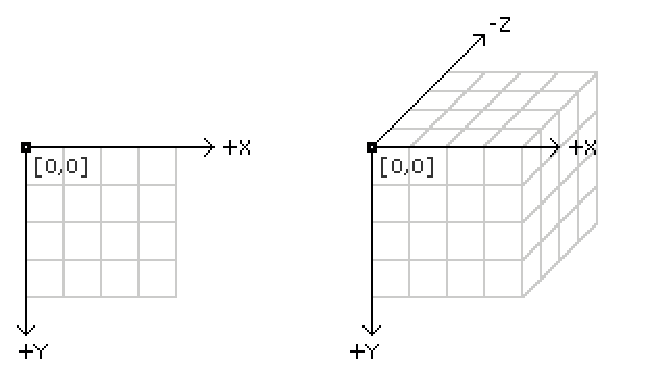
\includegraphics{images/coordinates.eps}
	\label{fig:coordinatesrato}
	\caption{O rato no sistema de coordenadas}
\end{figure}

\subsection{Posição}
A posição (x, y) do ponteiro do rato é actualizada e mantida em variáveis especiais do Processing. Estas variáveis são \texttt{mouseX} e \texttt{mouseY} (do tipo \texttt{int}) e são actualizadas constantemente pelo Processing. 

O programa seguinte (Exemplo~\ref{exe:interaccao_rato_xy}) exemplifica o uso destas variáveis.
\lstinputlisting[caption=Posição do Rato \\~% 
\texttt{[interaccao\_rato\_xy]}, label=exe:interaccao_rato_xy,%
firstline=10]{Interaccao//interaccao_rato_xy//interaccao_rato_xy.pde}

Podemos verificar que estas variáveis podem ser utilizadas como quaisquer outras variáveis, pelo que podemos passá-las como parâmetros de métodos, usá-las em expressões matemáticas, etc. 

\subsection{Botões}
O estado dos botões do rato pode ser obtido de duas formas. Podemos ``perguntar'' se um botão foi pressionado, ou podemos pedir ao Processing que nos informe sempre que um botão for pressionado.

Para a primeira forma, utilizamos a variável booleana \texttt{mousePressed} que indica se um botão está pressionado (a variável é \texttt{true} se um botão estiver pressionado e \texttt{false} se não estiver nenhum botão pressionado). Se a variável for \texttt{true}, então podemos utilizar a variável \texttt{mouseButton} para determinar qual o botão pressionado (o botão do lado esquerdo, do meio, ou da direita).

\lstinputlisting[caption=Botões do Rato Síncronos, label=exe:interaccao_rato_botoes_sincrono,%
firstline=10]{Interaccao//interaccao_rato_botoes_sincrono//interaccao_rato_botoes_sincrono.pde}

Esta forma de obter o estado dos botões é feita de forma síncrona, ou seja, o programa lê o estado dos botões do rato num ponto específico do programa. Se, quando o programa chegar ao ponto em que verifica o estado dos botões, nenhum botão estiver pressionado então não é detectado nenhum botão pressionado. Se o utilizador pressionar e largar um botão do rato enquanto o programa está a desenhar o rectângulo:
\lstinputlisting[nolol= true, firstline=26, lastline=26]%
{Interaccao//interaccao_rato_botoes_sincrono//interaccao_rato_botoes_sincrono.pde}
O programa não irá detectar este acontecimento, porque, quando chegar à linha de código que faz a verificação, o utilizador já largou o botão. Isto significa que se podem ``perder'' eventos do rato.

Para isto não acontecer, temos de obter o estado dos botões de forma assíncrona, ou seja, deixamos o Processing informar o programa sempre que um botão for pressionado. Desta forma, seja qual for o ponto em que o nosso programa estiver, os eventos são sempre detectados.
Para usarmos esta forma de obter o estado do rato permite-nos obter não só o estado dos botões mas também outros eventos do rato. Para isso utilizamos os métodos de \emph{callback} já descritos no Capítulo~\ref{cap:metodos}:

\begin{itemize}
\item \texttt{mousePressed()} -- invocado pelo Processing quando o utilizador clica num botão do rato.

\item \texttt{mouseMoved()} -- invocado pelo Processing quando o utilizador arrasta o rato.

\item \texttt{mouseDragged()} -- invocado pelo Processing quando o utilizador arrasta o rato mantendo um botão pressionado.

\item \texttt{mouseReleased()} --	invocado pelo Processing quando o utilizador larga um botão do rato.
\end{itemize}

O programa seguinte mostra como adaptar o Exemplo~\ref{exe:interaccao_rato_botoes_sincrono} para utilizar a nova forma de obter o estado dos botões.

\lstinputlisting[caption=Botões do Rato Assíncronos\\ \texttt{[interaccao\_rato\_botoes\_assincrono]}, label=exe:interaccao_rato_botoes_assincrono, firstline=10]{Interaccao//interaccao_rato_botoes_assincrono//interaccao_rato_botoes_assincrono.pde}


\section{O Teclado}
A obtenção do estado das teclas do teclado é feita de forma muito semelhante à utilizada para o rato.
Basicamente, temos os dois métodos descritos anteriormente: de forma síncrona e de forma assíncrona. 

A variável booleana \texttt{keyPressed} indica, à semelhança da variável \texttt{mousePressed} para o rato, se alguma tecla foi pressionada. A variável \texttt{key} contém o carácter associado à tecla pressionada. Para as teclas especiais, como as teclas direccionais, podemos utilizar a variável \texttt{keyCode} para verificar qual a tecla pressionada. O Exemplo~\ref{exe:interaccao_teclado_sincrono} mostra como ler as teclas pressionadas e o Exemplo~\ref{exe:interaccao_teclado_teclas_especiais} mostra como ler as teclas especiais.

\lstinputlisting[caption=Teclado \\ \texttt{[interaccao\_teclado\_sincrono]}, label=exe:interaccao_teclado_sincrono, firstline=10]{Interaccao//interaccao_teclado_sincrono//interaccao_teclado_sincrono.pde}


\lstinputlisting[caption=Teclado: Teclas Especiais \\ \texttt{[interaccao\_teclado\_teclas\_especiais]}, label=exe:interaccao_teclado_teclas_especiais, firstline=10]{Interaccao//interaccao_teclado_teclas_especiais//interaccao_teclado_teclas_especiais.pde}

Tal como no caso do rato, esta forma de ler o estado das teclas pode falhar se o utilizador pressionar e libertar a tecla antes de o programa chegar à instrução que lê o estado das teclas.

No entanto, se utilizarmos os métodos de \emph{callback}, garantimos que o programa recebe sempre os eventos do teclado.

Para o teclado, temos os métodos:
\begin{itemize}
\item \texttt{keyPressed()} -- invocado pelo Processing quando o utilizador carrega numa tecla do teclado. 

\item \texttt{keyReleased()} -- invocado pelo Processing quando o utilizador larga uma tecla do teclado. 
\end{itemize}

O exemplo seguinte mostra como utilizar estes métodos:
\lstinputlisting[caption=Teclado Assíncrono \\ \texttt{[interaccao\_teclado\_assincrono]}, label=exe:interaccao_teclado_assincrono, firstline=10]{Interaccao//interaccao_teclado_assincrono//interaccao_teclado_assincrono.pde}